\documentclass{article}
\usepackage{maa-monthly}

%% IF YOU HAVE FONTS INSTALLED
%\usepackage{mtpro2}
%\usepackage{mathtime}
\usepackage{subcaption}
%\theoremstyle{theorem}
\newtheorem{theorem}{Theorem}
\newtheorem{proposition}[theorem]{Proposition}
\newtheorem{lemma}[theorem]{Lemma}
\newtheorem{corollary}[theorem]{Corollary}

\theoremstyle{definition}
\newtheorem*{definition}{Definition}
\newtheorem*{remark}{Remark}

\begin{document}

\title{Flows and the Complex Ackermann Function}
\markright{Complex Ackermann Function}
\author{Author}

\maketitle

\begin{abstract}
The process of extending maps to flows is called continuous or fractional iteration. Extending tetration to the complex numbers is a classic example, finding functional square roots is another.

A general method of fractional iteration in the complex plane is presented based on Faà di Bruno's formula which decomposes the iterations of holomorphic functions into recursive Bell polynomials.

The classical Ackermann function along with fractional iteration defines an Ackermann function for complex numbers. 
\end{abstract}

\noindent

Consider the holomorphic function $f(z): \mathbb{C} \rightarrow \mathbb{C}$ and its iterates $f^t(z), t \in \mathbb{N}$ with a fixed point $L\in\mathbb{C}$ such that $f(L)=L$. The derivative of iterated function $D^nf^t(L)$ is $Df^t(L)=f'(L)^t$ and the most important factor in the dynamics of the map.

\section{Recursive Bell Polynomials}

\begin{theorem}[Recursive Bell Polynomial Theorem]
The derivatives of an iterated holomorphic function with a non-superattracting fixed point can be expressed in terms of recursive Bell polynomials.
$$D^nf^t(L)=\sum_{r=0}^\infty(\sum_{k=2}^n \frac{f^{(k)}(L)}{k!} B_{n,k}(D^2f^{t-1}(L),\ldots, D^{n-k+1}f^{t-1}(L)))^r$$
\end{theorem}

\begin{proof}
Consider the following version of Faà di Bruno's formula, \cite{weisstein}

${D^n} f(g(x)) = \sum_{k=1}^n f^{(k)}(g(x))\cdot B_{n,k}\left(g'(x),g''(x),\dots,g^{(n-k+1)}(x)\right)$.

Set $g(x)=f^{t-1}(x)$ and $x=L$,

$D^nf^t(L)=\sum_{k=1}^n \frac{f^{(k)}(L)}{k!} B_{n,k}(Df^{t-1}(L),\ldots, D^{n-k+1}f^{t-1}(L))$

By cases. There are two cases: $k<n$ and $k=n$.

Case 1. ($k<n$). $D^kf^{t-1}(L)$ is already known.

Case 2. ($k=n$). $D^nf^{t-1}(L)$ is not known but can be solved by a simple recursive expression resulting in the geometrical series where $C$ is a constant

$D^nf^t(x)=C+f'(L)D^nf^{t-1}(x)$.

By Taylor series $f^t(x)=\sum_{k=0}^\infty\frac{1}{k!} D^nf^t(L) (x - L)^k$
\end{proof}

\section{Flows}




\section{Ackermann Function}
The following is the original definition of the Ackermann function.

\begin{align}
\varphi(m, n, 0) &= m + n \\ \nonumber
\varphi(m, 0, 1) &= 0 \\ \nonumber
\varphi(m, 0, 2) &= 1 \\ \nonumber
\varphi(m, 0, p) &= m && \text{for } p > 2 \\ \nonumber
\varphi(m, n, p) &= \varphi(m, \varphi(m, n-1, p), p - 1) && \text{for } n, p > 0\nonumber
\end{align}

If $\varphi(m, z, p)$ converges then where $q>p$ the higher hyperoperators $\varphi(m, z, q)$ converge.

\subsection{Convergence}
Let $L$ be a fixed point in the exponential map of $a^x$ then $a^L=L$.

$${dz}\to\ln{L}\;{dz}$$

The action of a single iteration near a fixed point.

$$a^{L+dz}=a^L a^{dz}=L\;a^{dz}\approx L(1+\ln{a})=L+L\ln{a}\;{dz}=L+\ln{L}\;dz$$

Location of the fixed points of the roots of unity.
$$\ln{L}=e^{2 \pi i x}$$
$$L=e^{e^{2 \pi i x}}$$

Location of the of the base for a given fixed point.
$$w^{1/w}$$

The boundary of the Shell - Thron region of convergence of the exponential map of $a^z$
$$e^{2 i \pi  x e^{-2 i \pi  x}}$$

\begin{figure}[htp]
\centering
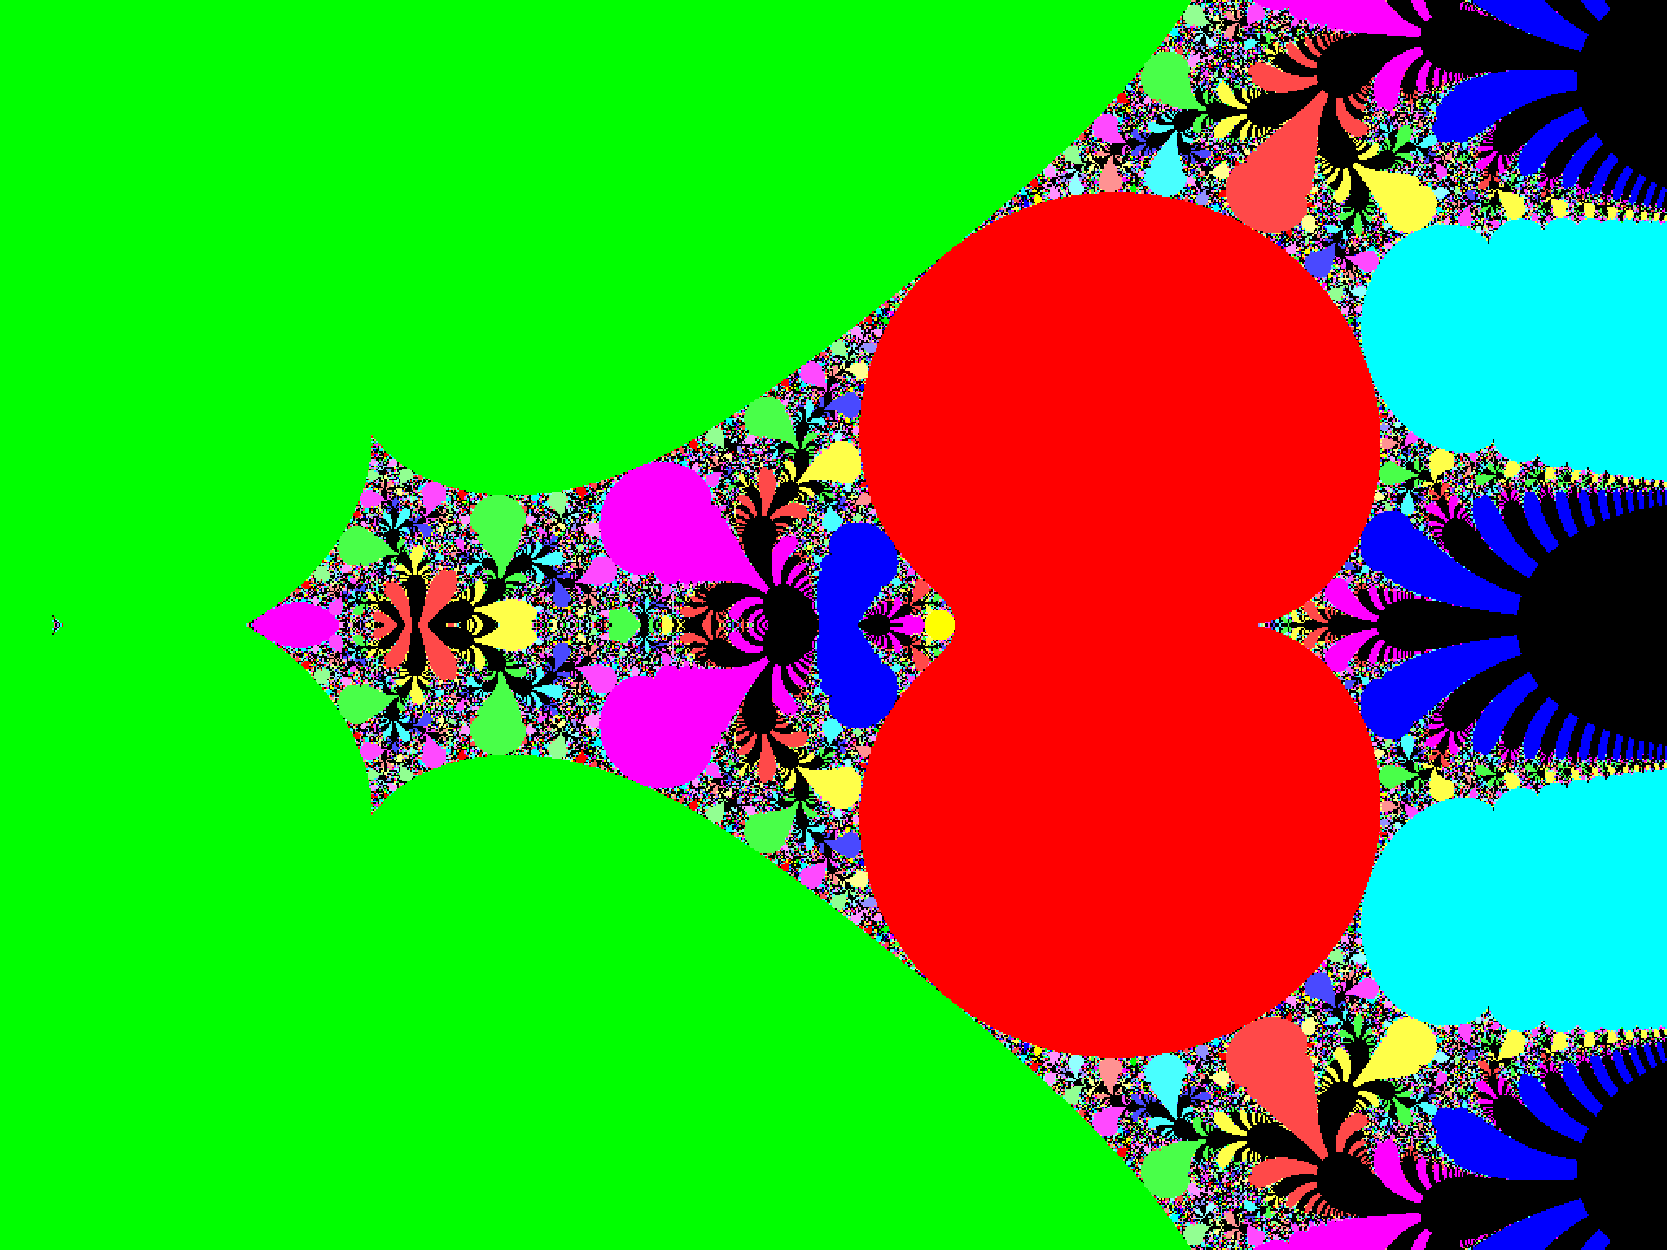
\includegraphics[width=0.25\textwidth]{period.png}
\caption{Tetration Period Fractal}
\label{fig:period}
\end{figure}

\begin{figure}[htp]
\centering
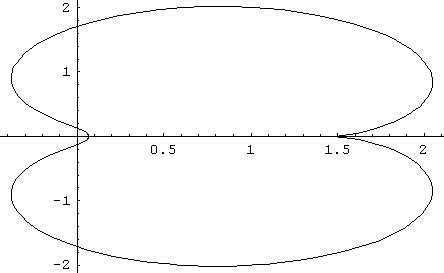
\includegraphics[width=0.25\textwidth, height=0.4\textwidth]{shell_thron.png}
\caption{Shell-Thron boundary}
\label{fig:shell-thron}
\end{figure}

Tetration period fractal
\begin{figure}[htp]
\centering
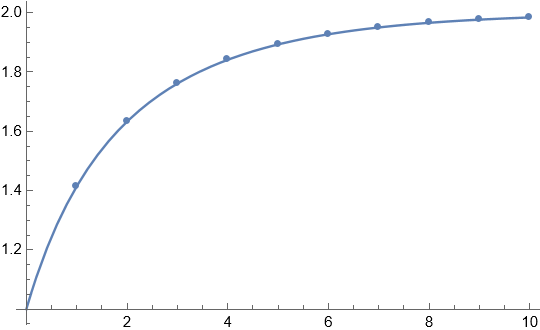
\includegraphics[width=0.25\textwidth]{Ackermann.png}
\caption{Discrete tetration of $\sqrt{2}^z$ compared with the tetration flow $^z(\sqrt{2})$}
\label{fig:tetration}
\end{figure}

\section{Mathematica code}
\begin{verbatim}
   Flow[f_, t_, x_, L_, order_ : 3] := Module[{s},
   H[0] = L;
   H[1] = f'[L]^t ;
   Do[H[max] = First[r[t] /. 
      RSolve[{r[0] == 0, r[t] ==
        Sum[Derivative[k][f][L] BellY[max, k,Table[H[j]
          /. t -> t - 1, {j, max}]], {k, 2, max}] 
        + f'[L] r[t - 1]}, r[t], t]], 
   {max, 2, order}];
   s = Sum[1/k! H[k] (x - L)^k, {k, 0, order}]
];
\end{verbatim}

\begin{acknowledgment}{Acknowledgment.}
The authors wish to thank the Greek polymath Anonymous, whose prolific works are an endless source of inspiration.
\end{acknowledgment}

\begin{thebibliography}{1}
\bibitem{weisstein} Weisstein, Eric W. "Faà di Bruno's Formula." From

\textit{MathWorld}--A Wolfram Web Resource. 

https://mathworld.wolfram.com/FaadiBrunosFormula.html
\end{thebibliography}


\vfill\eject

\end{document}
